\subsection{Story: Admins can create quizzes via the website}
\subsubsection{Analysis - breakdown of tasks}
This story is quite large and should be broken down into several substories:
\begin{itemize}
	\item (3) Admins can log into a backend
	\item (2) They are presented with a list of their quizzes
	\item (5) They can create a new quiz in the backend
	\item (3) They can edit an existing quiz they own
\end{itemize}
\newpage

\subsection{Story: Admins can log into the backend}
\subsubsection{Analysis - breakdown of tasks}
\begin{itemize}
	\item Create users table
	\item Add login page
	\item Add register page
\end{itemize}
\subsubsection{Design}
A use case diagram was produced to show the actions a lecturer has for this stage\ref{fig:login-use-case}.

\begin{figure}
	\caption{Use case diagram for the admin backend for login}
	\centerline{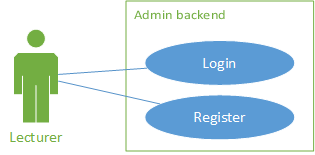
\includegraphics{Chapter2/Iter-1/iter-1-use-case}}
	\label{fig:login-use-case}
\end{figure}

\subsubsection{Implementation}
Implementing this was far easier than originally anticipated; Laravel comes with the required tables out of the box and has a command to run that sets up simple auth for users: \textit{php artisan make:auth} 
\subsubsection{Testing}
Because the login and auth is handled by Laravel by default, testing it was deemed not to be a priority. However, three simple tests were written to ensure it never breaks due to future changes.
\newpage

\subsection{Story: They are presented a list of their quizzes}
\subsubsection{Analysis - breakdown of tasks}
\begin{itemize}
	\item Make the homepage the QuizController rather than the HomeController
	\item Check and identify the user who is logged in
	\item Display a list of quizzes for that user
\end{itemize}
\subsubsection{Design}
The HomeController to be removed in this period of work and the QuizController used in its place. See figure \ref{fig:quiz-list-use-case} for the use case.

\begin{figure}
	\caption{Use case diagram for the admin backend including show quizzes}
	\centerline{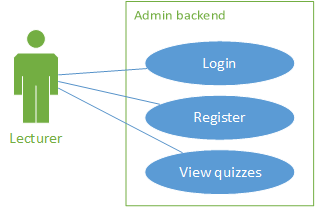
\includegraphics{Chapter2/Iter-1/iter-1-use-case-v2}}
	\label{fig:quiz-list-use-case}
\end{figure}

\subsubsection{Implementation}
Changing the controller was a small change to the routes and the quiz view file so that it used the same layout as the original home views. To get the user, a helper function is provided: \textit{auth()-$>$user()} which gets the user object. Obtaining the id from this is simple and then using an Eloquent ORM call it is easy to find all the quizzes owned by that user.
\subsubsection{Testing}
The tests written here highlighted a problem with the testing framework. For each test a new migration is made within the test database, thereby wiping the data created within each test. An unintended side effect however is that every new user created starts at id=1 in the users table (a user has to be created for all these tests.) Chrome is used as the Remote Web Driver for running these tests and seems to remember that the user of id=1 logged in in the previous test, and therefore skips the auth step. This means the test order is incorrect due to the test trying to log in even though it is already logged in. The solution to this was to create each new user in the next id record, whilst this was somewhat convoluted, it worked.
\newpage

\subsection{Non-story work}
\subsubsection{Database work}
Some initial work that is needed for almost all the stories is having a working database set up to store the users, quizzes, questions etc. Setting up the tables and their relationships was undertaken at the start because it was perceived that this would not take long.

While creating these tables it was possible to create the controllers needed within the application at the same time using: \textit{php artisan make:model *name* -mc } 
\subsubsection{Seed data}
Because of the amount of changes to the database that were being made, the tables were repeatedly wiped and seeding some data was needed. To do this some seeders were generated with \textit{php artisan make: seed *name*}. These were created under database/seeds/ and simply required creating new objects of the desired Model and adding the various fields as parameters of the objects. The objects are then saved to the database and the seeders can be run when a migration is called to generate this data.
\subsubsection{Layout changes}
The initial \textit{make:auth} command created a default home page with a menu bar and some basic styling. This styling was created with Bootstrap\cite{bootstrap} and is aesthetically pleasing so the basic styling has been kept. This layout was modified somewhat to add some menu options that persist across pages. This layout 
was then used by all the backend pages by extending it.
\newpage
